\documentclass[aspectratio=169,10pt]{beamer}

% ---------------------------------------------------------------------------
% Quantathon CR 2026 -- Challenge 3
% Presentacion de seguimiento: resultados del modelo de Fermi-Hubbard 2D
% (ladder 3x2) -- companera de presentacion_fermi_hubbard.tex (planteamiento)
% ---------------------------------------------------------------------------

\usetheme{Madrid}
\usecolortheme{default}
\setbeamertemplate{navigation symbols}{}
\setbeamertemplate{footline}[frame number]

\usepackage[utf8]{inputenc}
\usepackage[T1]{fontenc}
\usepackage{amsmath,amssymb}
\usepackage{braket}
\usepackage{booktabs}
\usepackage{graphicx}
\usepackage{tikz}
\usetikzlibrary{arrows.meta,positioning,decorations.pathreplacing,calc}

% ---- Paleta "cuantica" (identica a presentacion_fermi_hubbard.tex) -----
\definecolor{qDeep}{RGB}{35,32,90}
\definecolor{qMid}{RGB}{75,55,160}
\definecolor{qAccent}{RGB}{0,150,170}
\definecolor{qWarn}{RGB}{190,60,50}
\definecolor{qGray}{RGB}{90,90,95}

\setbeamercolor{structure}{fg=qMid}
\setbeamercolor{title}{fg=white,bg=qDeep}
\setbeamercolor{frametitle}{fg=white,bg=qDeep}
\setbeamercolor{palette primary}{fg=white,bg=qDeep}
\setbeamercolor{palette secondary}{fg=white,bg=qMid}
\setbeamercolor{palette tertiary}{fg=white,bg=qDeep}
\setbeamercolor{block title}{fg=white,bg=qMid}
\setbeamercolor{block body}{bg=qMid!8}
\setbeamercolor{block title alerted}{fg=white,bg=qWarn}
\setbeamercolor{block body alerted}{bg=qWarn!8}
\setbeamercolor{item}{fg=qAccent}
\setbeamerfont{frametitle}{series=\bfseries}

\newcommand{\good}[1]{\textcolor{qAccent}{\textbf{#1}}}
\newcommand{\warn}[1]{\textcolor{qWarn}{\textbf{#1}}}

\title[Fermi-Hubbard 2D: resultados]{Modelo de Fermi-Hubbard 2D en una escalera $3\times2$}
\subtitle{Resultados: ED, Trotter, error de Trotter y VQE}
\author{Quantathon CR 2026 -- QWorld Hackathon, Challenge 3}
\date{}

\begin{document}

% =============================================================
\begin{frame}
  \titlepage
\end{frame}

% =============================================================
\begin{frame}{Agenda}
  \tableofcontents
\end{frame}

\section{Recapitulacion}

% =============================================================
\begin{frame}{De la propuesta a los resultados}
  \begin{itemize}
    \item La presentacion anterior (\texttt{presentacion\_fermi\_hubbard.tex}) planteaba el
      problema: Hamiltoniano de Hubbard, mapeo Jordan-Wigner en una escalera $4\times2$
      (8 sitios, 16 qubits), capas de Trotter, y un plan de 4 secciones (A--D) espejo de TFIM.
    \item \good{Las 4 secciones, mas Limitaciones, ya estan implementadas} en
      \texttt{FermiHubbard2D\_ED\_Trotter\_VQE.ipynb} y verificadas de principio a fin.
    \item \warn{Un cambio importante respecto al plan original:} el notebook completo corre
      ahora sobre una escalera \textbf{$3\times2$} (6 sitios, 12 qubits), no $4\times2$ --
      la siguiente diapositiva explica por que.
  \end{itemize}
  \vspace{0.5em}
  \begin{block}{Esta presentacion cubre}
    Los resultados reales de cada seccion, las figuras que el notebook genera, y lo que
    salio distinto de lo planeado (incluyendo lo que \emph{no} convergio bien).
  \end{block}
\end{frame}

% =============================================================
\begin{frame}{Por que $3\times2$ y no $4\times2$}
  \begin{alertblock}{El VQE de la Seccion D fue quien obligo el cambio}
    Con el ansatz Hamiltoniano-Variacional a $4\times2$ (16 qubits), un angulo compartido por
    capa y COBYLA (igual que TFIM), \warn{no convergio} ni en el caso facil $U=0$
    (fermiones libres): mejor resultado $E=-5.28$ vs.\ el exacto $E=-12.00$, tras 150--300
    iteraciones. Un optimizador basado en gradiente ayudo poco y costo 24 minutos por corrida.
  \end{alertblock}
  \begin{block}{La solucion}
    A 12 qubits cada evaluacion de circuito cuesta $\sim$0.04s (vs.\ 0.3--0.7s a 16) --
    suficiente para dar \textbf{un angulo libre por enlace} (mas expresivo) y
    \textbf{varios reinicios aleatorios} de COBYLA por cada $U/t$, lo cual cierra
    \good{la mayor parte} (no toda) de la brecha. Se adopto $3\times2$ para \emph{todo} el
    notebook, no solo VQE, para mantener un solo sistema consistente.
  \end{block}
  \small Verificado como un problema genuino de costo/convergencia, no un error: se revisó a
  mano el Hamiltoniano y el circuito contra ED en el estado de referencia sin rotar.
\end{frame}

% =============================================================
\begin{frame}{Costo estructural del cambio: mas capas de Trotter, no menos}
  \begin{columns}[T]
    \begin{column}{0.5\textwidth}
      \textbf{Anillo de 4 sitios ($4\times2$):} \good{bipartito} -- sus 4 enlaces se
      2-colorean en grupos ``par''/``impar'' disjuntos $\Rightarrow$ 2 capas por pierna.
      \vspace{0.5em}

      \textbf{Anillo de 3 sitios ($3\times2$):} \warn{no bipartito} -- con solo 3 vertices,
      \emph{cualquier} par de sus 3 enlaces comparte un vertice $\Rightarrow$ cada
      \emph{posicion} de enlace necesita su propia capa.
    \end{column}
    \begin{column}{0.5\textwidth}
      \centering
      \renewcommand{\arraystretch}{1.3}
      \begin{tabular}{lcc}
        \toprule
         & $4\times2$ & $3\times2$ \\
        \midrule
        Sitios / qubits & 8 / 16 & 6 / 12 \\
        Dim.\ Hilbert & $2^{16}$ & $2^{12}$ \\
        Enlaces hopping & 24 & 18 \\
        Cadena $Z$ maxima & 3 qubits & 2 qubits \\
        \textbf{Capas Trotter} & \textbf{7} & \warn{\textbf{9}} \\
        \bottomrule
      \end{tabular}
    \end{column}
  \end{columns}
  \vspace{0.8em}
  \begin{block}{Conclusion}
    La red mas chica \good{no es uniformemente mas barata} -- es mas barata exactamente donde
    importaba (costo por circuito de VQE), pero mas cara en estructura de capas de Trotter.
  \end{block}
\end{frame}

\section{Seccion A -- ED (linea base)}

% =============================================================
\begin{frame}{Resultados: diagnosticos de crossover vs.\ $U/t$}
  \centering
  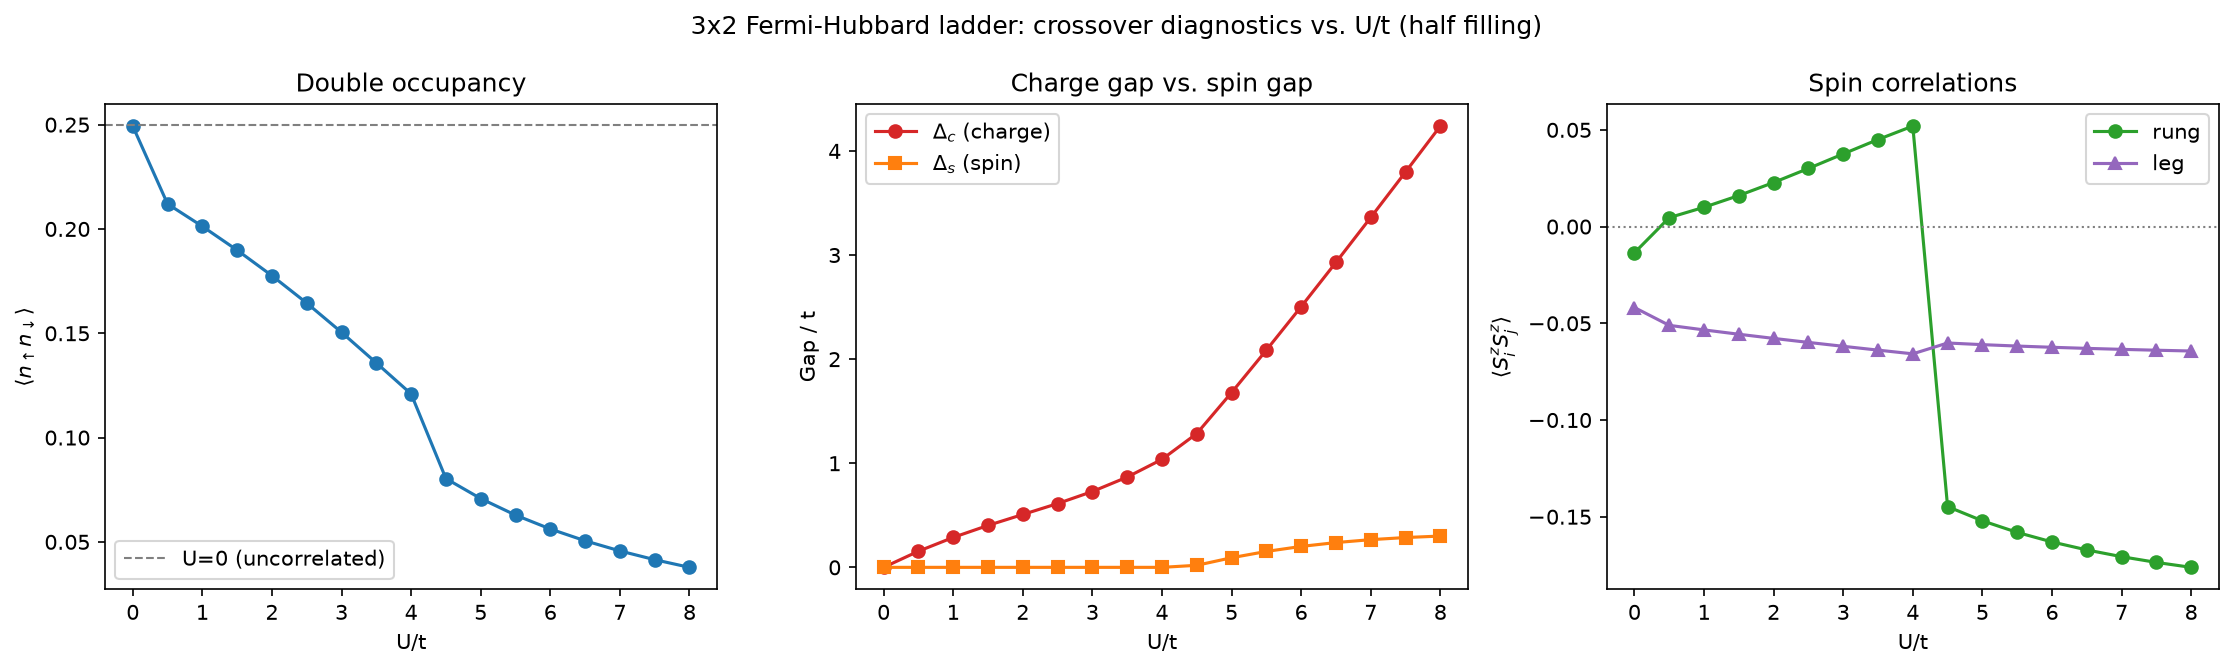
\includegraphics[width=\textwidth]{../fermi_hubbard_2d_phase_diagram.png}
  \vspace{0.3em}

  \small Barrido de 17 puntos, $U/t\in[0,8]$, sector de llenado medio
  ($N_\uparrow=N_\downarrow=3$, dimension $400$) -- corre en \good{menos de 1 segundo}.
\end{frame}

% =============================================================
\begin{frame}{Leyendo el crossover}
  \begin{itemize}
    \item \textbf{Doble ocupacion:} decrece suavemente de $1/4$ ($U=0$, no correlacionado) a
      $\sim$0.04 ($U/t=8$) -- la firma esperada de supresion de doble ocupacion.
    \item \textbf{Brecha de carga $\Delta_c$:} crece monotonicamente de $0$ a $\sim$4.2 --
      \good{positiva para todo $U>0$}, consistente con "gapeado siempre" (no hay $U_c$).
    \item \textbf{Brecha de espin $\Delta_s$:} mucho mas pequena, crece suavemente hasta
      $\sim$0.3 -- el diagnostico propio de la escalera (ausente en una cadena 1D).
    \item \warn{Artefacto de tamano finito:} la correlacion de peldano tiene un \textbf{salto
      discontinuo} cerca de $U/t\approx4.3$, mientras que $\Delta_c$, $\Delta_s$ y la doble
      ocupacion se mantienen suaves ahi mismo -- firma de un cruce de niveles entre dos
      estados casi degenerados con caracter de espin distinto, tipico de diagonalizacion
      exacta en sistemas muy pequenos. \textbf{No} es un error de codigo; no se investigo
      mas a fondo y se documenta como limitacion.
  \end{itemize}
\end{frame}

\section{Seccion B -- Trotter (Qiskit)}

% =============================================================
\begin{frame}{Protocolo: \emph{quench} de decaimiento de doblones}
  \begin{block}{No hay un campo tipo $h/J$ que apagar/encender en Hubbard}
    En su lugar: preparamos un estado de \textbf{onda de densidad de carga} -- la pierna
    $y{=}0$ completamente doblemente ocupada, la pierna $y{=}1$ vacia
    ($N_\uparrow=N_\downarrow=3$, doble ocupacion inicial $=0.5$) -- y dejamos evolucionar
    bajo $U/t$ fijo. Es el protocolo estandar de \textbf{decaimiento de doblones} usado en
    experimentos de atomos frios (p.\ ej.\ Strohmaier et al.\ 2010).
  \end{block}
  \begin{itemize}
    \item Circuito: \textbf{9 capas} de Trotter de primer orden (Lie-Trotter), factorizacion
      \emph{exacta} por enlace (los terminos $XX$ y $YY$ conmutan) -- el unico error de
      Trotter viene del orden entre capas.
    \item Referencia exacta: \texttt{expm\_multiply} dentro del sector de llenado medio
      (dimension 400) de la Seccion A -- circuito y referencia nunca salen de ese sector.
    \item Barrido: $U/t\in\{1,4,8\}$, $T_{\max}=5$, $N_{\text{steps}}=50$, 2000 shots/circuito.
  \end{itemize}
\end{frame}

% =============================================================
\begin{frame}{Resultado: $U/t=1$ (acoplamiento debil)}
  \centering
  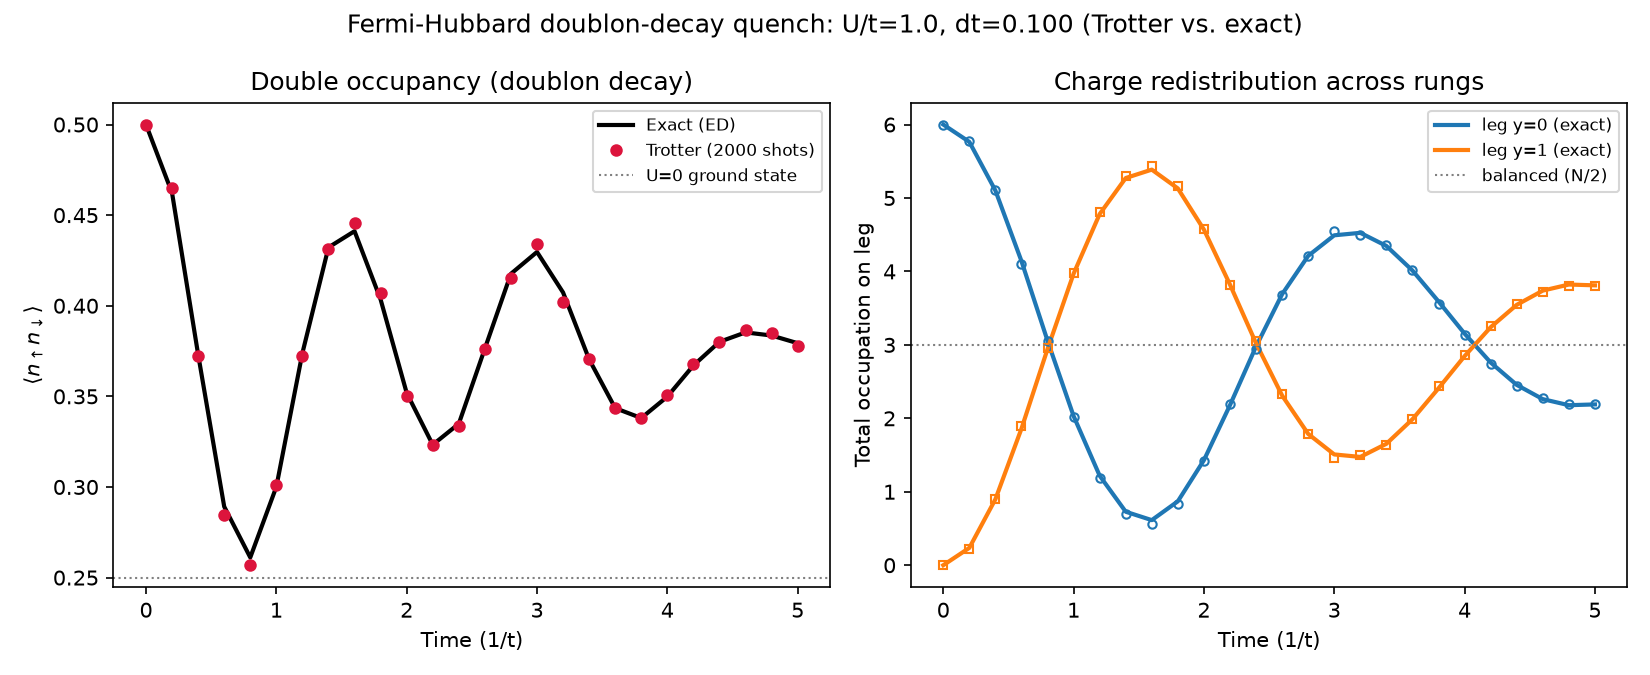
\includegraphics[width=0.92\textwidth]{../fermi_hubbard_quench_U1.0_trotter_vs_exact.png}
\end{frame}

% =============================================================
\begin{frame}{Resultado: $U/t=8$ (acoplamiento fuerte)}
  \centering
  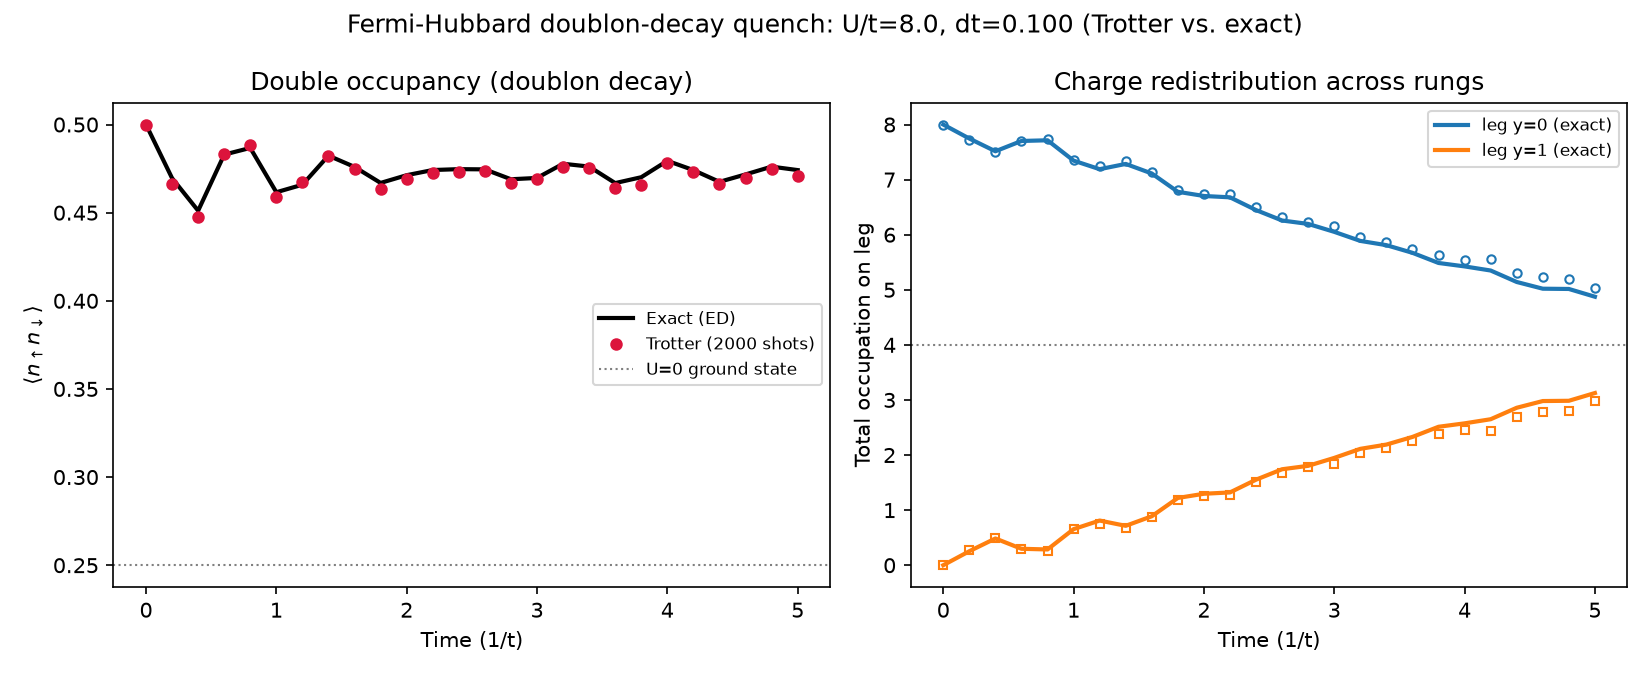
\includegraphics[width=0.92\textwidth]{../fermi_hubbard_quench_U8.0_trotter_vs_exact.png}
\end{frame}

% =============================================================
\begin{frame}{Leyendo el quench: supresion del decaimiento}
  \begin{itemize}
    \item \textbf{$U/t=1$:} la doble ocupacion oscila fuertemente (decae de 0.5 a $\sim$0.26 y
      rebota) -- hopping domina, el sistema "respira" entre las dos piernas con facilidad.
    \item \textbf{$U/t=8$:} la doble ocupacion apenas se mueve (se mantiene entre 0.46--0.50)
      -- \good{el decaimiento de doblones esta fuertemente suprimido}: la energia $U$
      liberada al decaer un doblon no tiene adonde ir de forma resonante. El transporte de
      carga de una sola particula \emph{si} sigue avanzando (panel derecho de cada figura)
      aunque la doble ocupacion casi no cambie.
    \item \warn{Esto es exactamente el fenomeno fisico esperado} (supresion de decaimiento de
      doblones a acoplamiento fuerte) -- el contraparte dinamico del crossover de la
      Seccion A, no una afirmacion fisica nueva.
    \item \good{Trotter vs.\ exacto:} la diferencia tipica es de $\sim$0.001--0.005 --
      consistente con ruido de shots (2000/circuito), no con error sistematico de Trotter.
  \end{itemize}
\end{frame}

\section{Seccion C -- Error de Trotter}

% =============================================================
\begin{frame}{Convergencia del error vs.\ $\Delta t$}
  \begin{columns}[T]
    \begin{column}{0.55\textwidth}
      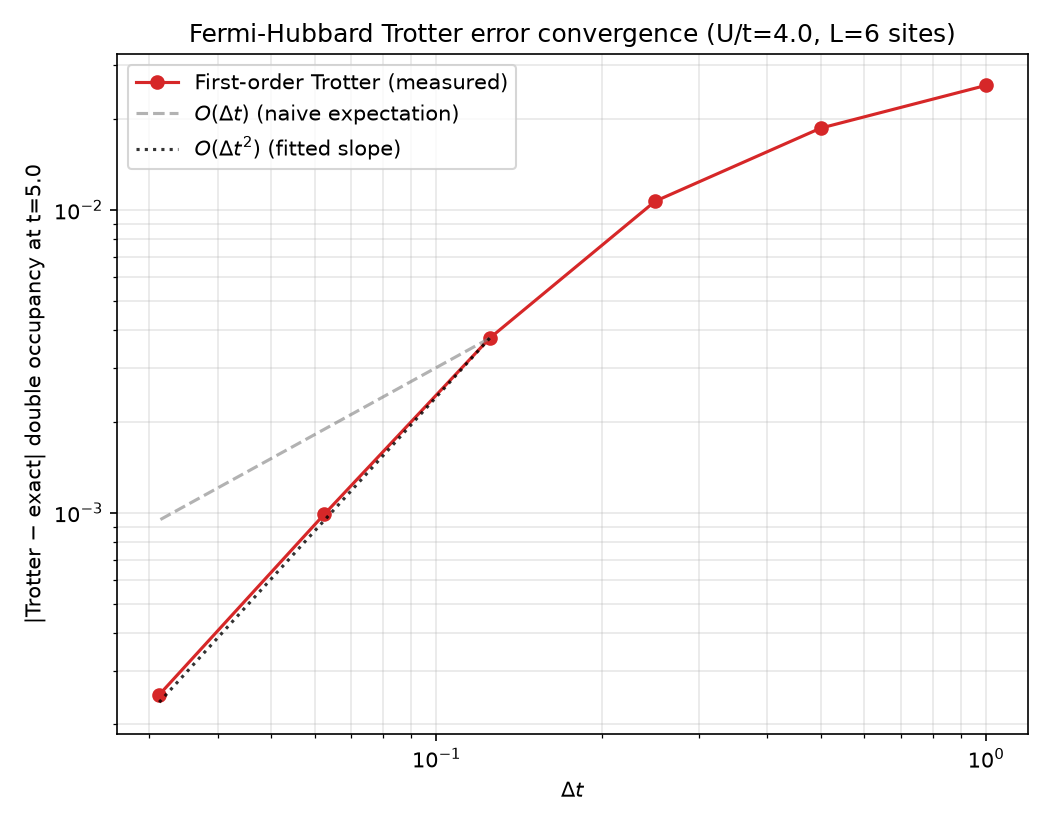
\includegraphics[width=\textwidth]{../fermi_hubbard_trotter_error_convergence.png}
    \end{column}
    \begin{column}{0.45\textwidth}
      \small
      \begin{itemize}
        \item $U/t=4$ fijo (escalas de hopping e interaccion comparables -- el peor caso
          para los conmutadores entre capas).
        \item Evaluacion \textbf{exacta} (sin shots) del \texttt{Statevector} -- a 2000
          shots el piso estadistico ($\sim1/\sqrt{N_{\text{shots}}L}$) enmascararia el
          error de Trotter justo donde hace falta resolverlo.
        \item $N_{\text{steps}}\in\{5,10,20,40,80,160\}$.
      \end{itemize}
    \end{column}
  \end{columns}
\end{frame}

% =============================================================
\begin{frame}{Un resultado medido, no forzado al valor de libro}
  \begin{alertblock}{Pendiente ajustada en el regimen asintotico ($n_{\text{steps}}\geq40$):
    $\mathbf{1.96}$}
    Mas pronunciada que el $O(\Delta t)$ \emph{global} esperado ingenuamente para un esquema
    de Trotter de primer orden (cuyo error \emph{local} es $O(\Delta t^2)$, que
    genericamente se acumula a $O(\Delta t)$ global).
  \end{alertblock}
  \begin{itemize}
    \item \good{No es casualidad de una sola red:} la misma pendiente ($1.98$) se midio de
      forma independiente al correr este mismo analisis sobre la red $4\times2$ original,
      con un numero distinto de capas (7, no 9) y un espacio de Hilbert completamente
      distinto.
    \item Explicacion honesta, no una prueba cerrada: el termino de error global de orden
      principal es una integral temporal de un conmutador anidado entre el estado y el
      observable -- puede ser anomalamente pequeno para combinaciones especificas de
      observable/estado/Hamiltoniano sin que el siguiente orden se suprima igual.
    \item Un esquema de segundo orden (Suzuki simetrico) se prototipo pero mostro error
      \emph{mayor} que primer orden en el mismo rango de $\Delta t$ -- no se resolvio en el
      tiempo disponible y se dejo fuera en vez de publicarse sin explicacion.
  \end{itemize}
\end{frame}

\section{Seccion D -- VQE}

% =============================================================
\begin{frame}{Ansatz: Hamiltoniano-Variacional, no Hardware-Efficient}
  \begin{block}{Reutiliza las mismas compuertas que Trotter (Secciones B/C)}
    Compuertas de hopping ($XX{+}YY$) e interaccion ($ZZ$), pero con \textbf{cada angulo
    como parametro libre} en vez de un angulo de Trotter fisicamente fijo -- aplicado al
    mismo estado de referencia (onda de densidad de carga) de las Secciones B/C.
  \end{block}
  \begin{itemize}
    \item \good{Conserva $N_\uparrow$/$N_\downarrow$ exactamente} para \emph{cualquier} valor
      de los parametros (las compuertas de hopping conservan numero por espin; la de
      interaccion es diagonal) -- tambien conserva $S_z$ exactamente (no necesariamente
      $S^2_{\text{tot}}$).
    \item $N_{\text{layers}}=2$, un angulo por enlace (ambos espines) mas uno por sitio de
      interaccion $=$ \textbf{48 parametros}.
    \item \texttt{run\_vqe}: 3 reinicios aleatorios de COBYLA (\texttt{maxiter=600}), se
      conserva el mejor -- necesario empiricamente, no opcional (ver diapositiva anterior
      sobre $4\times2$).
    \item Evaluacion de energia \textbf{exacta} via \texttt{Statevector.expectation\_value}
      (mas rapida que \texttt{Estimator} en este tamano de circuito, mismo resultado).
  \end{itemize}
\end{frame}

% =============================================================
\begin{frame}{Resultado: VQE vs.\ ED, barrido en $U/t$}
  \centering
  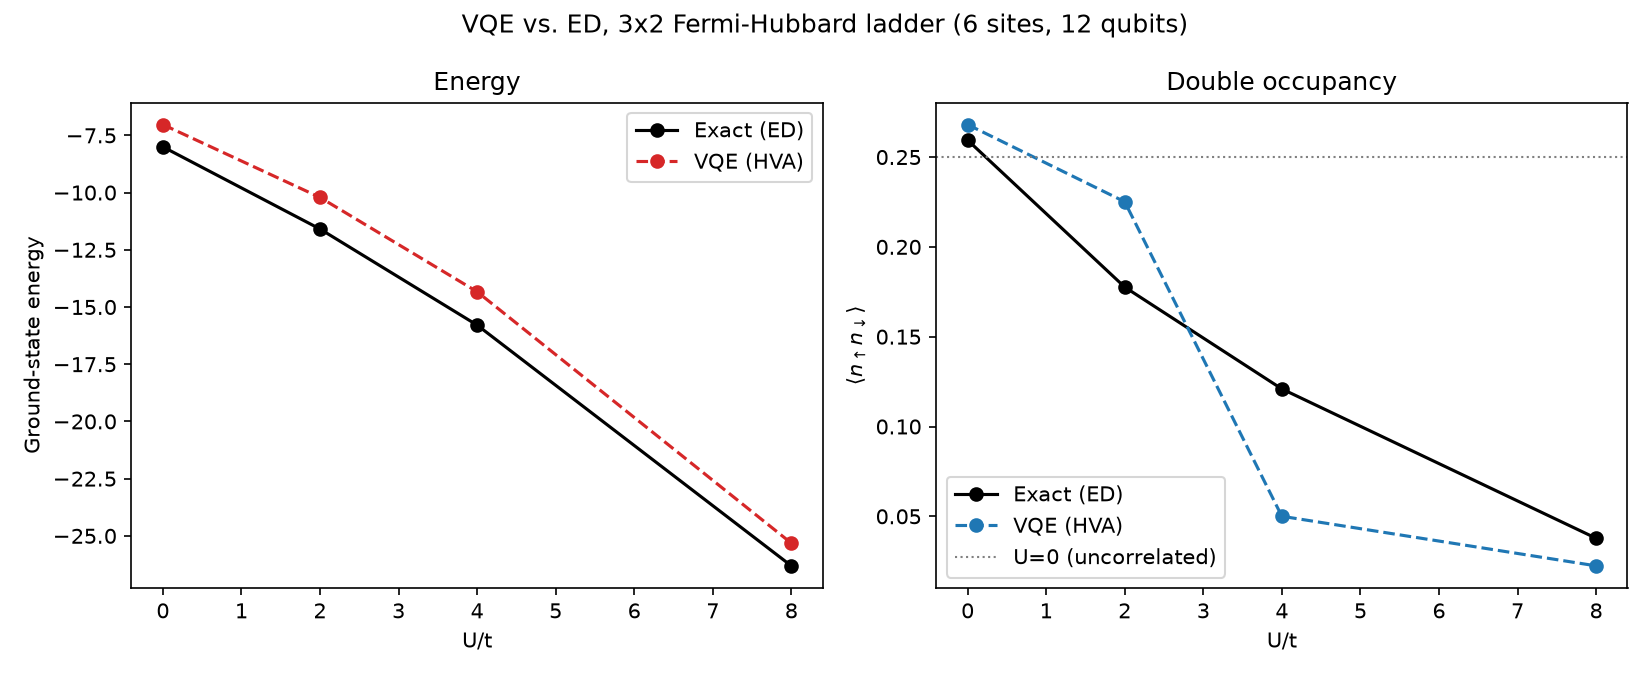
\includegraphics[width=\textwidth]{../fermi_hubbard_vqe_vs_ed.png}
\end{frame}

% =============================================================
\begin{frame}{Leyendo la comparacion: honesto, no pulido}
  \begin{itemize}
    \item VQE captura la \good{tendencia cualitativa correcta}: energia decrece y doble
      ocupacion cae desde el valor no correlacionado $0.25$ al aumentar $U/t$.
    \item \warn{Brecha persistente en energia}, $\sim$4--12\% relativo:
      $U/t{=}0$: $+0.97$; $U/t{=}2$: $+1.38$; $U/t{=}4$: $+1.46$; $U/t{=}8$: $+0.99$.
    \item \warn{Doble ocupacion, peor y con signo inconsistente:} VQE \emph{sobreestima} a
      $U/t{=}2$ ($0.225$ vs.\ $0.178$, muy poca correlacion) pero \emph{se pasa hacia abajo}
      a $U/t{=}4,8$ ($0.050$ vs.\ $0.121$; $0.022$ vs.\ $0.038$) -- cruza la curva exacta
      cerca de $U/t\sim3$.
    \item Consistente con lo visto antes: COBYLA con reinicios multiples \textbf{no}
      garantiza el optimo global a un presupuesto de iteraciones costeable.
    \item \good{No se persiguio mas} (mas reinicios/\texttt{maxiter}, gradiente via
      parameter-shift) para mantener el tiempo de ejecucion de esta seccion en el orden de
      minutos -- pasos legitimos, pero no implementados aqui.
  \end{itemize}
\end{frame}

\section{Limitaciones y cierre}

% =============================================================
\begin{frame}{Limitaciones honestas}
  \begin{itemize}
    \item \textbf{Tamano finito, crossover no transicion.} $N=6$, espacio de Hilbert
      $2^{12}{=}4096$ -- gapeado para todo $U>0$; nada aqui extrapola al limite
      termodinamico.
    \item \textbf{La red es un compromiso, no el plan original.} $3\times2$ en vez de
      $4\times2$, forzado por VQE -- con el costo estructural de 9 capas de Trotter, no 7.
    \item \textbf{Error de Trotter solo de primer orden}, verificado en un solo acoplamiento
      ($U/t=4$); el esquema de segundo orden prototipado no se resolvio a tiempo.
    \item \textbf{Secciones C y D evitan deliberadamente ruido de shots} -- solo la Seccion B
      simula el regimen de muestreo finito realista.
    \item \textbf{Simulador ideal, no hardware real} -- sin modelo de ruido, sin apendice de
      nube (a diferencia del notebook de TFIM).
    \item \textbf{Brecha de VQE cuantificada, no hipotetica} -- los numeros exactos estan en
      la Seccion D.4 del notebook.
    \item \textbf{Sobrecosto de Jordan-Wigner en 2D}: 18 terminos de hopping, de los cuales
      10 cargan cadenas de $Z$ (longitud 1 o 2) -- mas CNOTs por capa que cualquier enlace 1D.
  \end{itemize}
\end{frame}

% =============================================================
\begin{frame}{Resumen}
  \begin{itemize}
    \item El notebook de Fermi-Hubbard 2D esta \good{completo}: ED, Trotter, error de
      Trotter y VQE, con una seccion de Limitaciones honesta -- igual que TFIM.
    \item El cambio de red ($4\times2\to3\times2$) fue una decision \good{forzada
      empiricamente y documentada}, no una simplificacion silenciosa.
    \item Los resultados muestran \good{fisica correcta y reconocible}: crossover suave,
      supresion de decaimiento de doblones a $U/t$ grande, convergencia de Trotter medible.
    \item El VQE funciona pero \warn{no converge completamente} -- se reporta la brecha real,
      no un resultado pulido para verse mejor de lo que es.
  \end{itemize}
  \vfill
  \centering \large \textcolor{qDeep}{\textbf{Gracias -- preguntas}}
\end{frame}

\end{document}
